%% Manuscript for Industrial & Engineering Chemistry Research (ACS)
%% Class: achemso (journal = iecred), two-column layout.
%% Compile:  pdflatex manuscript; bibtex manuscript; pdflatex manuscript; pdflatex manuscript
%% Every number in the text is a macro from generated_numbers.tex and every table
%% body comes from generated_tables.tex; both are written by Codes/run_all.py.
\documentclass[journal=iecred,manuscript=article,layout=twocolumn]{achemso}
%% journal-like page: 10 pt type; the class sets a 7 in text block in two columns
\makeatletter\input{size10.clo}\makeatother
\geometry{letterpaper,top=16mm,bottom=20mm,left=19.3mm,right=19.3mm,columnsep=0.3in}
\usepackage{amsmath,amssymb,booktabs,multirow,graphicx,array}
\renewcommand{\topfraction}{0.92}\renewcommand{\dbltopfraction}{0.92}
\renewcommand{\bottomfraction}{0.6}\renewcommand{\textfraction}{0.06}
\renewcommand{\floatpagefraction}{0.85}\renewcommand{\dblfloatpagefraction}{0.85}
\setcounter{topnumber}{3}\setcounter{dbltopnumber}{3}\setcounter{totalnumber}{5}
\usepackage{tikz}
\usetikzlibrary{arrows.meta,positioning}
\usepackage[colorlinks=true,allcolors=black]{hyperref}
% GENERATED by Codes/run_all.py -- do not edit.  Every number quoted in the
% manuscript is one of these macros; Data/manuscript_numbers.csv gives its source.
\newcommand{\NDerivTotal}{336}% number of reduced derivatives
\newcommand{\NDerivNoS}{142}% derivatives that do not need S
\newcommand{\NDerivAllSeven}{96}% derivatives needing all seven symbols
\newcommand{\NDerivChecked}{672}% derivative checks performed (two states)
\newcommand{\NDerivSkipped}{0}% derivative checks skipped
\newcommand{\DerivMaxDevSC}{1.5 \times 10^{-5}}% max relative deviation, PR supercritical
\newcommand{\DerivMedDevSC}{1.3 \times 10^{-9}}% median relative deviation, PR supercritical
\newcommand{\DerivNBelowSC}{324}% count below 1e-6, PR supercritical
\newcommand{\DerivMaxDevGas}{8.9 \times 10^{-6}}% max relative deviation, PR gas
\newcommand{\DerivMedDevGas}{2.8 \times 10^{-10}}% median relative deviation, PR gas
\newcommand{\DerivNBelowGas}{324}% count below 1e-6, PR gas
\newcommand{\NMaxwell}{4}% Maxwell relations confirmed
\newcommand{\NRecip}{336}% reciprocity identities confirmed
\newcommand{\NCyclic}{336}% cyclic-rule identities confirmed
\newcommand{\ClosedNumMax}{5.4 \times 10^{-10}}% max closed-form vs numerical difference
\newcommand{\ClosedNumN}{144}% number of closed-form vs numerical comparisons
\newcommand{\ConsistMax}{2.7 \times 10^{-9}}% max residual of G and H surface identities
\newcommand{\ConsistN}{45}% number of consistency comparisons
\newcommand{\PRCritResid}{8.6 \times 10^{-5}}% PR critical-pressure residual
\newcommand{\PRrhoAAD}{1.8}% PR density AAD %, all CO2 points
\newcommand{\PRrhoMax}{10}% PR density max deviation %
\newcommand{\SRKrhoAAD}{3.3}% SRK density AAD %, all CO2 points
\newcommand{\SRKrhoMax}{17}% SRK density max deviation %
\newcommand{\RKrhoAAD}{2.1}% RK density AAD %, all CO2 points
\newcommand{\RKrhoMax}{15}% RK density max deviation %
\newcommand{\vdWrhoAAD}{4.7}% vdW density AAD %, all CO2 points
\newcommand{\vdWrhoMax}{27}% vdW density max deviation %
\newcommand{\IGrhoAAD}{22.3}% IG density AAD %, all CO2 points
\newcommand{\IGrhoMax}{75}% IG density max deviation %
\newcommand{\PRrhoAADlow}{0.6}% PR density AAD %, 0.1-4 MPa
\newcommand{\PRrhoAADmid}{2.1}% PR density AAD %, 6-10 MPa
\newcommand{\PRrhoAADhigh}{3.6}% PR density AAD %, 15-20 MPa
\newcommand{\PRCpAAD}{2.7}% PR Cp AAD %
\newcommand{\PRCpMax}{21}% PR Cp max %
\newcommand{\PRCvAAD}{5.0}% PR Cv AAD %
\newcommand{\PRwAAD}{2.4}% PR sound speed AAD %
\newcommand{\PRmuAAD}{8.5}% PR Joule-Thomson AAD %
\newcommand{\PRdHAAD}{104}% PR enthalpy-change AAD, J/mol
\newcommand{\PRdSAAD}{0.24}% PR entropy-change AAD, J/(mol K)
\newcommand{\SRKrhoAADlow}{0.2}% SRK density AAD %, 0.1-4 MPa
\newcommand{\SRKrhoAADmid}{2.8}% SRK density AAD %, 6-10 MPa
\newcommand{\SRKrhoAADhigh}{10.3}% SRK density AAD %, 15-20 MPa
\newcommand{\SRKCpAAD}{2.3}% SRK Cp AAD %
\newcommand{\SRKCpMax}{18}% SRK Cp max %
\newcommand{\SRKCvAAD}{4.0}% SRK Cv AAD %
\newcommand{\SRKwAAD}{4.2}% SRK sound speed AAD %
\newcommand{\SRKmuAAD}{5.2}% SRK Joule-Thomson AAD %
\newcommand{\SRKdHAAD}{66}% SRK enthalpy-change AAD, J/mol
\newcommand{\SRKdSAAD}{0.19}% SRK entropy-change AAD, J/(mol K)
\newcommand{\IGdHAAD}{2878}% ideal-gas enthalpy-change AAD, J/mol
\newcommand{\vdWCvAAD}{11.8}% vdW Cv AAD %
\newcommand{\IGCvAAD}{11.8}% ideal-gas Cv AAD %
\newcommand{\PRPsatAAD}{0.5}% PR saturation pressure AAD %
\newcommand{\PRrhoLAAD}{4.4}% PR saturated liquid density AAD %
\newcommand{\SRKPsatAAD}{0.5}% SRK saturation pressure AAD %
\newcommand{\SRKrhoLAAD}{12.6}% SRK saturated liquid density AAD %
\newcommand{\RKPsatAAD}{19.5}% RK saturation pressure AAD %
\newcommand{\RKrhoLAAD}{16.0}% RK saturated liquid density AAD %
\newcommand{\vdWPsatAAD}{73.7}% vdW saturation pressure AAD %
\newcommand{\vdWrhoLAAD}{38.4}% vdW saturated liquid density AAD %
\newcommand{\PRdHvapAAD}{2.4}% PR enthalpy of vaporisation AAD %
\newcommand{\PRdHvapMax}{13}% PR enthalpy of vaporisation max %
\newcommand{\PRrhoVAAD}{1.1}% PR saturated vapour density AAD %
\newcommand{\NtwoPRrhoAAD}{2.4}% N2 PR density AAD %
\newcommand{\NtwoPRCpAAD}{0.6}% N2 PR Cp AAD %
\newcommand{\NtwoPRwAAD}{3.0}% N2 PR sound speed AAD %
\newcommand{\NtwoSRKrhoAAD}{1.3}% N2 SRK density AAD %
\newcommand{\NtwoSRKCpAAD}{1.1}% N2 SRK Cp AAD %
\newcommand{\NtwoSRKwAAD}{1.0}% N2 SRK sound speed AAD %
\newcommand{\TabdHAAD}{57}% table route enthalpy AAD, J/mol
\newcommand{\TabdSAAD}{0.18}% table route entropy AAD, J/(mol K)
\newcommand{\TabdHAADlow}{10}% table route enthalpy AAD 0.1-4 MPa, J/mol
\newcommand{\TabdHMax}{1379}% table route enthalpy max, J/mol
\newcommand{\TabCpAAD}{19}% table route Cp AAD %
\newcommand{\TabCvAAD}{54}% table route Cv AAD %
\newcommand{\TabCpAADlow}{12}% table route Cp AAD %, 0.1-4 MPa
\newcommand{\TabHeldCpAADlow}{2.0}% held-out table Cp AAD %, 0.1-4 MPa
\newcommand{\TabHeldrhoAAD}{0.10}% held-out table density AAD %
\newcommand{\TabHeldrhoMax}{3.6}% held-out table density max %
\newcommand{\TabHelddHAAD}{52}% held-out table enthalpy AAD, J/mol
\newcommand{\TabNRefused}{6}% grid nodes refused by the table route (kappaT <= 0)
\newcommand{\TabNNodes}{171}% grid nodes tested, full table
\newcommand{\NNistCOtwo}{171}% CO2 single-phase reference points
\newcommand{\NNistTotal}{200}% all NIST reference state points
\newcommand{\NScen}{17}% number of scenarios
\newcommand{\NScenOK}{8}% scenarios completing normally
\newcommand{\NScenPartial}{3}% scenarios with partial results
\newcommand{\NScenIncons}{1}% scenarios flagged inconsistent
\newcommand{\NScenError}{5}% scenarios refused with an error
\newcommand{\InfCv}{38.33}% Cv inferred from stated measurements
\newcommand{\InfCvU}{0.24}% its standard uncertainty
\newcommand{\InfCvNist}{38.325}% NIST Cv at 350 K, 10 MPa
\newcommand{\InfKappaT}{0.1582}% inferred kappaT, 1/MPa
\newcommand{\InfAlpha}{10.553}% inferred alpha, 1e-3 /K
\newcommand{\TabScendH}{-5822}% table scenario enthalpy change, J/mol
\newcommand{\TabScendS}{-51.96}% table scenario entropy change
\newcommand{\TabScendHNist}{-5828}% NIST enthalpy change for the same states
\newcommand{\TabScendSNist}{-51.98}% NIST entropy change for the same states
\newcommand{\SatP}{4.160}% PR saturation pressure at 280 K, MPa
\newcommand{\SatPU}{0.006}% its standard uncertainty, MPa
\newcommand{\SatPNist}{4.1607}% NIST saturation pressure at 280 K, MPa
\newcommand{\OneRho}{5.277}% PR molar density at 350 K, 10 MPa, mol/L
\newcommand{\OneRhoNist}{5.1989}% NIST density at 350 K, 10 MPa
\newcommand{\OneCp}{82.66}% PR Cp at 350 K, 10 MPa
\newcommand{\OneCpNist}{85.729}% NIST Cp at 350 K, 10 MPa
\newcommand{\OneCpU}{0.16}% its standard uncertainty
\newcommand{\OneMu}{6.145}% PR Joule-Thomson coefficient, K/MPa
\newcommand{\OneMuU}{0.006}% its standard uncertainty
\newcommand{\MCRatioMin}{0.99}% min Monte Carlo / linear u
\newcommand{\MCRatioMax}{1.03}% max Monte Carlo / linear u
\newcommand{\MCN}{36}% outputs compared
\newcommand{\TwodH}{-12634}% process enthalpy change, J/mol
\newcommand{\TwodHU}{16}% its standard uncertainty
\newcommand{\TwodS}{-73.72}% process entropy change
\newcommand{\TwodSU}{0.10}% its standard uncertainty
\newcommand{\TwodHShareTtwo}{76}% share of T2 in var(dH), %
\newcommand{\TwodHShareOmega}{10}% share of omega in var(dH), %
\newcommand{\TwodSSharePone}{74}% share of P1 in var(dS), %
\newcommand{\TwodSShareTtwo}{19}% share of T2 in var(dS), %
\newcommand{\InfCvShareCp}{47}% share of Cp in var(Cv), %
\newcommand{\InfCvShareMu}{40}% share of muJT in var(Cv), %
\newcommand{\NTests}{81}% tests passed
\newcommand{\NTestsFailed}{0}% tests failed
\newcommand{\PyVer}{3.12.3}% Python version used
\newcommand{\NumpyVer}{2.5.4}% NumPy version used
\newcommand{\ScipyVer}{1.18.1}% SciPy version used
\newcommand{\MplVer}{3.11.2}% Matplotlib version used
\newcommand{\NCodeLines}{2548}% lines in the engine package

% GENERATED by Codes/run_all.py from the CSV files in Data/ -- do not edit.
\newcommand{\TabDiffBody}{%
$T$ & $1$ & $0$ \\
$P$ & $0$ & $1$ \\
$V$ & $V \alpha$ & $-V \kappa_T$ \\
$S$ & $\frac{C_P}{T}$ & $-V \alpha$ \\
$U$ & $C_P - P V \alpha$ & $V\left(P \kappa_T - T \alpha\right)$ \\
$H$ & $C_P$ & $V\left(1 - T \alpha\right)$ \\
$A$ & $-\left(P V \alpha + S\right)$ & $P V \kappa_T$ \\
$G$ & $-S$ & $V$ \\
}
\newcommand{\TabDerivBody}{%
$\left(\partial T/\partial P\right)_{H}$ & $\displaystyle \frac{V\left(T \alpha - 1\right)}{C_P}$ & $T, V, C_P, \alpha$ \\[4pt]
$\left(\partial T/\partial P\right)_{S}$ & $\displaystyle \frac{T V \alpha}{C_P}$ & $T, V, C_P, \alpha$ \\[4pt]
$\left(\partial U/\partial V\right)_{T}$ & $\displaystyle \frac{T \alpha - P \kappa_T}{\kappa_T}$ & $T, P, \alpha, \kappa_T$ \\[4pt]
$\left(\partial H/\partial P\right)_{T}$ & $\displaystyle V\left(1 - T \alpha\right)$ & $T, V, \alpha$ \\[4pt]
$\left(\partial S/\partial V\right)_{T}$ & $\displaystyle \frac{\alpha}{\kappa_T}$ & $\alpha, \kappa_T$ \\[4pt]
$\left(\partial T/\partial V\right)_{U}$ & $\displaystyle \frac{T \alpha - P \kappa_T}{T V \alpha^{2} - C_P \kappa_T}$ & $T, P, V, C_P, \alpha, \kappa_T$ \\[4pt]
$\left(\partial P/\partial T\right)_{V}$ & $\displaystyle \frac{\alpha}{\kappa_T}$ & $\alpha, \kappa_T$ \\[4pt]
$\left(\partial S/\partial T\right)_{V}$ & $\displaystyle \frac{C_P \kappa_T - T V \alpha^{2}}{T \kappa_T}$ & $T, V, C_P, \alpha, \kappa_T$ \\[4pt]
$\left(\partial G/\partial P\right)_{T}$ & $\displaystyle V$ & $V$ \\[4pt]
$\left(\partial A/\partial V\right)_{T}$ & $\displaystyle -P$ & $P$ \\[4pt]
$\left(\partial H/\partial S\right)_{P}$ & $\displaystyle T$ & $T$ \\[4pt]
$\left(\partial U/\partial S\right)_{V}$ & $\displaystyle T$ & $T$ \\[4pt]
}
\newcommand{\TabEosBody}{%
vdW & $0$ & $0$ & 0.42188 & 0.12500 & $1$ \\
RK & $0$ & $1$ & 0.42748 & 0.08664 & $T_r^{-1/2}$ \\
SRK & $0$ & $1$ & 0.42748 & 0.08664 & $[1+m(1-T_r^{1/2})]^2$ \\
PR & $1-\sqrt{2}$ & $1+\sqrt{2}$ & 0.45724 & 0.07780 & $[1+m(1-T_r^{1/2})]^2$ \\
}
\newcommand{\TabFluidBody}{%
carbon dioxide & 44.0095 & 304.1282 & 7.3773 & 0.22394 & 24.99735 & 55.18696 & -33.69137 & 7.94839 & -0.136638 & 298--1200 \\
nitrogen & 28.0134 & 126.1920 & 3.3958 & 0.03720 & 28.98641 & 1.85398 & -9.64746 & 16.63537 & 0.000117 & 100--500 \\
}
\newcommand{\TabValBody}{%
\multirow{5}{*}{0.1--4} & IG & 5.4 & 3.2 & 8.4 & 3.0 & 100.0 & 526 & 1.10 \\
 & vdW & 0.4 & 3.2 & 4.7 & 0.8 & 21.9 & 144 & 0.42 \\
 & RK & 0.3 & 1.8 & 2.1 & 0.5 & 5.1 & 42 & 0.15 \\
 & SRK & 0.2 & 1.5 & 0.8 & 0.6 & 4.3 & 17 & 0.06 \\
 & PR & 0.6 & 1.8 & 0.9 & 0.1 & 9.4 & 41 & 0.07 \\
\midrule
\multirow{5}{*}{6--10} & IG & 28.2 & 16.2 & 43.7 & 13.9 & 100.0 & 3138 & 7.07 \\
 & vdW & 4.9 & 16.2 & 17.1 & 6.2 & 9.6 & 697 & 2.11 \\
 & RK & 2.5 & 8.5 & 7.8 & 2.4 & 3.7 & 240 & 0.83 \\
 & SRK & 2.8 & 7.8 & 3.0 & 6.6 & 2.9 & 92 & 0.31 \\
 & PR & 2.1 & 9.0 & 3.6 & 3.5 & 5.3 & 172 & 0.36 \\
\midrule
\multirow{5}{*}{15--20} & IG & 47.2 & 22.1 & 61.9 & 15.3 & 100.0 & 7189 & 16.14 \\
 & vdW & 12.8 & 22.1 & 38.4 & 9.2 & 35.9 & 1901 & 5.82 \\
 & RK & 5.1 & 4.3 & 14.6 & 4.2 & 7.2 & 739 & 2.35 \\
 & SRK & 10.3 & 3.2 & 4.1 & 7.6 & 10.6 & 123 & 0.26 \\
 & PR & 3.6 & 5.5 & 5.3 & 5.5 & 11.4 & 129 & 0.39 \\
\midrule
\multirow{5}{*}{all} & IG & 22.3 & 11.8 & 32.1 & 9.4 & 100.0 & 2878 & 6.43 \\
 & vdW & 4.7 & 11.8 & 16.3 & 4.5 & 20.9 & 719 & 2.18 \\
 & RK & 2.1 & 4.6 & 6.8 & 1.9 & 5.1 & 263 & 0.86 \\
 & SRK & 3.3 & 4.0 & 2.3 & 4.2 & 5.2 & 66 & 0.19 \\
 & PR & 1.8 & 5.0 & 2.7 & 2.4 & 8.5 & 104 & 0.24 \\
}
\newcommand{\TabValNtwoBody}{%
1--31 & IG & 5.0 & 3.9 & 15.7 & 13.4 & 100.0 & 638 & 2.23 \\
 & vdW & 3.5 & 3.9 & 3.4 & 2.3 & 37.5 & 100 & 0.13 \\
 & RK & 2.0 & 1.8 & 1.2 & 3.2 & 10.5 & 25 & 0.27 \\
 & SRK & 1.3 & 3.3 & 1.1 & 1.0 & 11.4 & 49 & 0.02 \\
 & PR & 2.4 & 1.8 & 0.6 & 3.0 & 13.5 & 80 & 0.05 \\
}
\newcommand{\TabSatBody}{%
vdW & 73.7 & 38.4 & 89.9 & 55.4 \\
RK & 19.5 & 16.0 & 22.0 & 20.3 \\
SRK & 0.5 & 12.6 & 1.3 & 2.9 \\
PR & 0.5 & 4.4 & 1.1 & 2.4 \\
}
\newcommand{\TabRouteBody}{%
\multicolumn{7}{@{}l}{\emph{all 19 temperatures, evaluated at the nodes}} \\
0.1--4 & 0.001 & 17 & 12 & 2 & 10 & 0.03 \\
6--10 & 0.001 & 51 & 14 & 10 & 55 & 0.17 \\
15--20 & 0.002 & 146 & 46 & 19 & 175 & 0.53 \\
\multicolumn{7}{@{}l}{\emph{10 K spacing, evaluated at held-out nodes}} \\
0.1--4 & 0.001 & 3 & 2 & 0 & 6 & 0.02 \\
6--10 & 0.277 & 19 & 5 & 4 & 51 & 0.16 \\
15--20 & 0.007 & 66 & 20 & 28 & 167 & 0.50 \\
}
\newcommand{\TabScenBody}{%
01 & state & state, 3 derivatives, uncertainty & completed \\
02 & process & process, uncertainty & completed \\
03 & saturation & saturation at 280 K & completed \\
04 & derivative & 12 derivatives, symbolic only & completed \\
05 & infer & inference from stated $V$, $C_P$, $w$, $\mu_{JT}$ & completed \\
06 & infer & $\alpha$ not supplied & partial result; missing input named \\
07 & infer & stated $C_V > C_P$ & flagged inconsistent \\
08 & table & process from tabulated $V(T,P)$ & completed \\
09 & table & 450 K requested, table ends at 400 K & refused: out-of-range error \\
10 & state & $P$ given in kelvin & refused: unit error \\
11 & state & $T$ given without a unit & refused: unit error \\
12 & state & user fluid without $C_P^{\circ}$ & partial result; missing input named \\
13 & state & 250 K, below $C_P^{\circ}$ range & refused: out-of-range error \\
14 & state & N$_2$, SRK, $^\circ$C and bar input & completed \\
15 & state & ideal gas, tabulated $C_P^{\circ}$ & completed \\
16 & state & fluid not in database & refused: missing-data error \\
17 & state & $(\partial P/\partial T)_H$ in an ideal gas & partial result; singular derivative reported \\
}
\newcommand{\TabBudgetBody}{%
$\Delta h$ (J mol$^{-1}$) & -12634 & 16 & 7 & 0 & 76 & 4 & 2 & 1 & 10 \\
$\Delta s$ (J mol$^{-1}$ K$^{-1}$) & -73.72 & 0.10 & 1 & 74 & 19 & 2 & 0 & 0 & 3 \\
$\Delta u$ (J mol$^{-1}$) & -10277 & 14 & 5 & 0 & 73 & 6 & 2 & 1 & 13 \\
$\Delta g$ (J mol$^{-1}$) & 11875 & 34 & 0 & 96 & 3 & 0 & 0 & 0 & 0 \\
}

\newcommand{\pd}[3]{\left(\frac{\partial #1}{\partial #2}\right)_{\!#3}}
\newcommand{\Cpo}{C_P^{\circ}}
\setlength{\emergencystretch}{2em}

%% ---- AUTHORS: replace every [TO FILL] entry; do not leave placeholders in a submission
\author{[Author One -- TO FILL]}
\author{[Author Two -- TO FILL]}
\author{[Author Three -- TO FILL]}
\author{[Author Four -- TO FILL]}
\author{[Author Five -- TO FILL]}
\email{[corresponding.author@institute -- TO FILL]}
\affiliation{[Group name, Department, Institute, City, Postal code, Country -- TO FILL]}

\title{A Computational Engine for the Calculus of Thermodynamics: Exact Derivative
Reduction, Computability Analysis, and Equation-of-State Evaluation with
Uncertainty}

\begin{document}

\begin{abstract}
We describe a small open engine that carries out the calculus of thermodynamics
for a pure simple fluid. It reduces every first derivative
$(\partial X/\partial Y)_Z$ among $T$, $P$, $V$, $S$, $U$, $H$, $A$, and $G$
(\NDerivTotal{} cases) exactly to measurable quantities, decides from the data
supplied whether a target is computable, names the missing inputs when it is
not, flags inconsistent inputs, and propagates input uncertainty. All reduced
formulas agree with direct numerical differentiation to better than
$\DerivMaxDevSC$ in relative terms. Against NIST reference data for carbon
dioxide (310--400~K, 0.1--20~MPa) the Peng--Robinson equation gives densities
with an average absolute deviation of \PRrhoAAD\% and enthalpy changes within
\PRdHAAD~J~mol$^{-1}$; tabulated volumes alone reproduce enthalpy changes within
\TabdHAAD~J~mol$^{-1}$ on average but do not give reliable heat capacities.
\end{abstract}

\section{Introduction}

Thermodynamic analysis repeatedly asks the same question in different clothes:
how does one property change with a second while a third is held fixed, and can
the answer be evaluated from what is actually known? The formal answer has been
available for more than a century. Bridgman tabulated the first derivatives of
the common state functions of a simple system,\cite{Bridgman1914} and
Shaw\cite{Shaw1935} showed that the whole table follows from Jacobian algebra;
both treatments are standard textbook material.\cite{Callen1985,Smith2018} What
the tables do not provide is a decision procedure for a practical problem, in
which some quantities are measured, some are read from tables, some come from
an equation of state (EoS), and some are simply missing.

Mature property software addresses a different need. CoolProp\cite{Bell2014}
and the NIST databases\cite{NISTWebBook} evaluate multiparameter reference
equations, such as those of Span and Wagner for carbon
dioxide\cite{Span1996} and of Span et al.\ for nitrogen,\cite{Span2000} with
an accuracy that cubic equations cannot approach, and they return many
derivatives of the Helmholtz energy directly. They assume, however, that a
complete model of the fluid exists; they do not reason about partial
information, and their inner workings are not meant to be read by a student.
Computer algebra has been used to derive and code thermodynamic models
automatically,\cite{Castier1999} and departure-function calculations with cubic
equations remain common in engineering studies, for example for
refrigerant--oil mixtures\cite{MarcelinoNeto2013} and
propellants.\cite{daSilva2023} These works automate the derivation or the
evaluation of a chosen model, not the question of whether a requested quantity
is determined by the available data.

This paper describes an engine built for that question. Its contributions are
modest in theory and practical in kind: (i) an exact, dependency-free reduction
of all \NDerivTotal{} first derivatives of eight state variables to $T$, $P$,
$V$, $S$, $C_P$, the expansivity $\alpha$, and the isothermal compressibility
$\kappa_T$; (ii) a rule-based analysis that infers what follows from the given
data, reports the smallest sets of additional inputs that would make a target
computable, and detects contradictory inputs; (iii) uniform treatment of stated,
tabulated, inferred, and parameterized inputs, with provenance attached to every
result; (iv) first-order propagation of input uncertainty with a Monte Carlo
check; and (v) a verification and validation record in which every number is
regenerated from the code. Nothing in items (i) and (iv) is new science, and
the equations of state used are the classical cubic
ones.\cite{vanderWaals1873,Redlich1949,Soave1972,Peng1976} The engine is not a
replacement for reference-quality property libraries; it is a transparent tool
for analysis and teaching whose failure modes are stated explicitly.

\section{Theory and Methodology}

\subsection{Fundamental Relations and Potentials}

For a closed, simple compressible system the fundamental relation
$\mathrm{d}U = T\,\mathrm{d}S - P\,\mathrm{d}V$ and the Legendre transforms
$H = U + PV$, $A = U - TS$, and $G = H - TS$ give\cite{Callen1985}
\begin{equation}
\begin{aligned}
\mathrm{d}H &= T\,\mathrm{d}S + V\,\mathrm{d}P, &
\mathrm{d}A &= -S\,\mathrm{d}T - P\,\mathrm{d}V,\\
\mathrm{d}G &= -S\,\mathrm{d}T + V\,\mathrm{d}P. &&
\end{aligned}
\label{eq:potentials}
\end{equation}
Equality of mixed second derivatives of $U$, $H$, $A$, and $G$ yields the four
Maxwell relations. The engine works with molar quantities and with three
measurable response functions,
\begin{equation}
\begin{gathered}
C_P = T\pd{S}{T}{P},\qquad
\alpha = \frac{1}{V}\pd{V}{T}{P},\\
\kappa_T = -\frac{1}{V}\pd{V}{P}{T}.
\end{gathered}
\label{eq:response}
\end{equation}

\subsection{Reduction of Derivatives}

Taking $(T,P)$ as independent variables, eqs~\ref{eq:potentials} and
\ref{eq:response} and the Maxwell relation
$(\partial S/\partial P)_T = -(\partial V/\partial T)_P$ give the two partial
derivatives of each of the eight variables listed in
Table~\ref{tab:diff}. Any derivative then follows from the Jacobian
identity\cite{Shaw1935}
\begin{equation}
\begin{gathered}
\pd{X}{Y}{Z} = \frac{J(X,Z)}{J(Y,Z)},\\
J(X,Z) = X_T Z_P - X_P Z_T ,
\end{gathered}
\label{eq:jacobian}
\end{equation}
where subscripts $T$ and $P$ denote the entries of Table~\ref{tab:diff}. The
result is a ratio of polynomials in the seven symbols $T$, $P$, $V$, $S$, $C_P$,
$\alpha$, and $\kappa_T$. The engine represents such ratios exactly, as Laurent
polynomials with rational coefficients, and brings them to a normal form by
cancelling the common monomial and numerical content and by exact polynomial
division when one polynomial divides the other. No computer algebra system is
required. A general multivariate greatest-common-divisor step is not
implemented; the correctness of every result is established numerically below,
but minimality of the printed form is not proved. Table~\ref{tab:deriv} shows
representative results together with the symbols each one needs. The set of
symbols is the basis of the computability decision: of the \NDerivTotal{}
derivatives, \NDerivNoS{} do not involve the entropy and can therefore be
evaluated from volumetric and caloric measurements alone, whereas
\NDerivAllSeven{} need all seven symbols.

\begin{table}
\caption{Partial Derivatives in the $(T,P)$ Plane Used in eq~\ref{eq:jacobian}}
\label{tab:diff}
\small
\resizebox{\columnwidth}{!}{%
\begin{tabular}{lll}
\toprule
$X$ & $(\partial X/\partial T)_P$ & $(\partial X/\partial P)_T$ \\
\midrule
\TabDiffBody
\bottomrule
\end{tabular}}
\end{table}

\begin{table}
\caption{Selected Reduced Derivatives Produced by the Engine and the Symbols
Each Requires}
\label{tab:deriv}
\small
\resizebox{\columnwidth}{!}{%
\begin{tabular}{@{}l@{\hspace{4pt}}l@{\hspace{4pt}}l@{}}
\toprule
derivative & reduced form & needs \\
\midrule
\TabDerivBody
\bottomrule
\end{tabular}}
\end{table}

A derivative does not exist where $J(Y,Z)$ vanishes. The engine evaluates the
denominator, compares it with the magnitude of its terms, and reports a
singular derivative instead of dividing; $(\partial P/\partial T)_H$ in an ideal
gas, for which $T\alpha = 1$, is the standard example.

\subsection{Heat Capacities and Related Identities}

Applying eq~\ref{eq:jacobian} to $C_V = T(\partial S/\partial T)_V$ gives
$C_P - C_V = TV\alpha^2/\kappa_T$; similarly the isentropic compressibility is
$\kappa_S = \kappa_T - TV\alpha^2/C_P = \kappa_T C_V/C_P$, the Joule--Thomson
coefficient is $\mu_{JT} = V(T\alpha - 1)/C_P$, the thermal pressure coefficient
is $(\partial P/\partial T)_V = \alpha/\kappa_T$, and the speed of sound is
$w = (V/M\kappa_S)^{1/2}$ with $M$ the molar mass. These identities, with the
definition of the compressibility factor $Z = PV/RT$, form the rule base used
for inference.

\subsection{Equations of State and Residual Functions}

Parameterized volumetric input is supplied by the ideal-gas law or by a cubic
equation written in the generic form\cite{Smith2018,Poling2001}
\begin{equation}
P = \frac{RT}{V-b} - \frac{a(T)}{(V+\epsilon b)(V+\sigma b)},
\label{eq:cubic}
\end{equation}
with $a(T) = \Omega_a \alpha_c(T_r) R^2T_c^2/P_c$ and $b = \Omega_b RT_c/P_c$.
Table~\ref{tab:eos} lists the constants for the van der Waals
(vdW),\cite{vanderWaals1873} Redlich--Kwong (RK),\cite{Redlich1949}
Soave--Redlich--Kwong (SRK),\cite{Soave1972} and Peng--Robinson
(PR)\cite{Peng1976} equations. With
$q(V) = \int_V^\infty \mathrm{d}V'/[(V'+\epsilon b)(V'+\sigma b)]$, the residual
Helmholtz energy at the temperature and volume of the fluid is
\begin{equation}
A^R(T,V) = -RT\ln\!\left(1-\frac{b}{V}\right) - a(T)\,q(V),
\label{eq:AR}
\end{equation}
from which $S^R = -(\partial A^R/\partial T)_V$, $U^R = A^R + TS^R$, and
$C_V^R = -T(\partial^2 A^R/\partial T^2)_V$ follow in closed form; conversion
to residuals at the same $T$ and $P$ adds $R\ln Z$ to the entropy and
$PV - RT$ to the enthalpy. The real-fluid enthalpy and entropy are
\begin{align}
H &= \int_{T_0}^{T}\Cpo\,\mathrm{d}T + H^R(T,P), \label{eq:H}\\
S &= \int_{T_0}^{T}\frac{\Cpo}{T}\,\mathrm{d}T - R\ln\frac{P}{P_0} + S^R(T,P),
\label{eq:S}
\end{align}
with the ideal gas at $T_0 = 298.15$~K and $P_0 = 1$~bar as the zero of both.
The ideal-gas heat capacity $\Cpo(T)$ is a Shomate polynomial with the
coefficients of the NIST--JANAF tables,\cite{Chase1998,NISTWebBook} a constant,
or a table; each form carries its range of validity. At a given $T$ and $P$
all admissible volume roots of eq~\ref{eq:cubic} are found and the root of
lowest fugacity is taken as stable; the saturation pressure is obtained by
equating the fugacities of the liquid and vapor roots, bracketed between the
spinodal pressures. Critical constants, acentric factors, molar masses, and
$\Cpo$ coefficients (Table~\ref{tab:fluids}) were taken from the NIST Chemistry
WebBook.\cite{NISTWebBook,Span1996,Span2000,Chase1998}

\begin{table}
\caption{Constants of the Cubic Equations of State in eq~\ref{eq:cubic}$^a$}
\label{tab:eos}
\footnotesize
\setlength{\tabcolsep}{3.5pt}
\begin{tabular}{@{}llllll@{}}
\toprule
EoS & $\epsilon$ & $\sigma$ & $\Omega_a$ & $\Omega_b$ & $\alpha_c(T_r)$ \\
\midrule
\TabEosBody
\bottomrule
\end{tabular}

\raggedright\footnotesize $^a$ $m = 0.480 + 1.574\omega - 0.176\omega^2$ for
SRK\cite{Soave1972} and $m = 0.37464 + 1.54226\omega - 0.26992\omega^2$ for
PR;\cite{Peng1976} $T_r = T/T_c$.
\end{table}

\begin{table*}
\caption{Fluid Constants and Ideal-Gas Heat Capacity Coefficients Used by the
Engine$^a$}
\label{tab:fluids}
\small
\resizebox{\textwidth}{!}{%
\begin{tabular}{lcccccccccc}
\toprule
fluid & $M$ (g mol$^{-1}$) & $T_c$ (K) & $P_c$ (MPa) & $\omega$ & $A$ & $B$ & $C$ &
$D$ & $E$ & range (K) \\
\midrule
\TabFluidBody
\bottomrule
\end{tabular}}

\raggedright\footnotesize $^a$ $\Cpo = A + Bt + Ct^2 + Dt^3 + E/t^2$ in
J~mol$^{-1}$~K$^{-1}$ with $t = T/(1000~\mathrm{K})$. Values as given by the
NIST Chemistry WebBook.\cite{NISTWebBook}
\end{table*}

\subsection{Differentiation and Integration Scheme}

A second, model-independent route accepts any pressure-explicit function
$P(T,V)$. First and second derivatives are central differences with one
Richardson extrapolation step (error of order $h^4$; relative steps of
$10^{-3}$ and $10^{-2}$), and the residual Helmholtz energy is the
Gauss--Kronrod quadrature
\begin{equation}
\frac{A^R(T,V)}{RT} = \int_0^{\rho}\frac{Z-1}{\rho'}\,\mathrm{d}\rho',
\qquad \rho = 1/V ,
\label{eq:quad}
\end{equation}
with a relative tolerance of $10^{-12}$; $S^R$ and $C_V^R$ follow by numerical
differentiation of eq~\ref{eq:quad} with respect to temperature. This scheme
makes user-supplied models usable and provides an independent check of the
closed forms.

Tabulated $P$--$V$--$T$ input on a rectangular $(T,P)$ grid is converted to
$Z(T,P)$ and fitted with an interpolating bicubic tensor-product spline.
Derivatives come from the spline, and residual functions from
\begin{align}
H^R &= -RT^2\!\int_0^P\!\pd{Z}{T}{P}\frac{\mathrm{d}P}{P}, \label{eq:HRtab}\\
S^R &= -R\!\int_0^P\!\left[Z-1+T\pd{Z}{T}{P}\right]\frac{\mathrm{d}P}{P}.
\label{eq:SRtab}
\end{align}
Because a table does not reach zero pressure, the integrands are taken as
constant below the lowest tabulated pressure, which is exact for a fluid that
obeys the second-virial form $Z - 1 \propto P$ there; the size of this
correction is reported with every result. The engine never extrapolates a
table.

\subsection{Inputs, Provenance, Computability, and Missing Data}

Every quantity known to the engine carries one of four provenances:
\emph{stated} (given with a unit), \emph{tabulated} (interpolated from a user
table), \emph{parameterized} (evaluated from an EoS or a $\Cpo$ correlation), or
\emph{inferred} (derived through an exact identity). Inputs are written as a
number and a unit; a small dimensional parser converts them to SI and rejects a
missing unit or a unit of the wrong dimension.

The identities of the preceding subsection are stored as directed rules, each
giving one quantity from others. Forward chaining applies every rule whose
inputs are known until no new quantity appears (Figure~\ref{fig:arch}). A target
is \emph{computable} if it is then known; a derivative is computable if every
symbol of its reduced form is known. If a target is not computable, a backward
search over the same rules returns the smallest sets of additional quantities
that would make it so, and these are reported to the user. When a rule
reproduces a quantity that is already known, the two values are compared: a
relative difference above a user tolerance (default 1\%) is reported as an
inconsistency, as are violations of the stability conditions $\kappa_T > 0$,
$\kappa_S > 0$, $C_V > 0$, and $C_P \ge C_V$.

\begin{figure*}
\centering
\resizebox{\textwidth}{!}{%
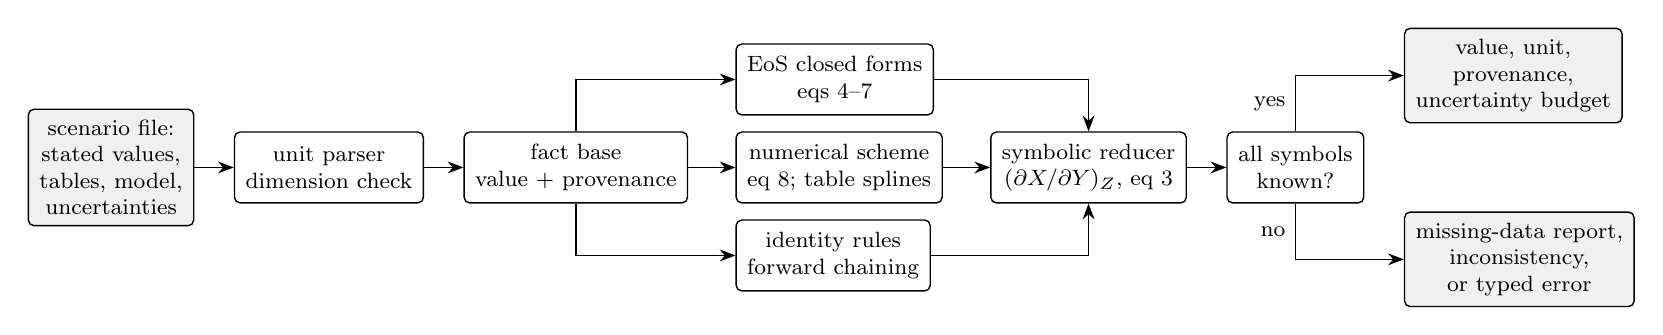
\begin{tikzpicture}[font=\footnotesize, node distance=4mm and 5mm,
  box/.style={draw, rounded corners=2pt, align=center, inner sep=4pt,
              minimum height=9mm, line width=0.5pt},
  io/.style={box, fill=black!6},
  arr/.style={-{Stealth[length=2mm]}, line width=0.5pt}]
\node[io] (in) {scenario file:\\stated values,\\tables, model,\\uncertainties};
\node[box, right=of in] (units) {unit parser\\dimension check};
\node[box, right=of units] (facts) {fact base\\value + provenance};
\node[box, above right=2mm and 6mm of facts] (eos) {EoS closed forms\\eqs 4--7};
\node[box, right=6mm of facts] (num) {numerical scheme\\eq 8; table splines};
\node[box, below right=2mm and 6mm of facts] (rules) {identity rules\\forward chaining};
\node[box, right=6mm of num] (sym) {symbolic reducer\\$(\partial X/\partial Y)_Z$, eq 3};
\node[box, right=of sym, align=center] (dec) {all symbols\\known?};
\node[io, above right=1mm and 5mm of dec] (ok) {value, unit,\\provenance,\\uncertainty budget};
\node[io, below right=1mm and 5mm of dec] (miss) {missing-data report,\\inconsistency,\\or typed error};
\draw[arr] (in) -- (units);
\draw[arr] (units) -- (facts);
\draw[arr] (facts) |- (eos);
\draw[arr] (facts) -- (num);
\draw[arr] (facts) |- (rules);
\draw[arr] (eos) -| (sym);
\draw[arr] (num) -- (sym);
\draw[arr] (rules) -| (sym);
\draw[arr] (sym) -- (dec);
\draw[arr] (dec) |- node[pos=0.25, left] {yes} (ok);
\draw[arr] (dec) |- node[pos=0.25, left] {no} (miss);
\end{tikzpicture}}
\caption{Architecture of the engine. Inputs of any provenance enter a common
fact base; parameterized models, the numerical scheme, and identity rules add
facts; the symbolic reducer states which facts a requested derivative needs,
and the result is either a value with its uncertainty budget or a statement of
what is missing or inconsistent.}
\label{fig:arch}
\end{figure*}

\subsection{Propagation of Input Uncertainty}

For an output $y = f(x_1,\dots,x_n)$ with uncorrelated inputs of standard
uncertainty $u(x_i)$, the engine applies the first-order law of
propagation,\cite{GUM2008}
\begin{equation}
u^2(y) = \sum_{i}\left(\frac{\partial f}{\partial x_i}\right)^{\!2}u^2(x_i),
\label{eq:gum}
\end{equation}
with sensitivities from central differences of the complete calculation
(relative step $10^{-5}$), and reports the fraction of $u^2(y)$ contributed by
each input. Uncertain inputs may be state variables, stated measurements, or
model parameters ($T_c$, $P_c$, $\omega$). A Monte Carlo propagation with
independent normal inputs can be requested as a check on the linearization.
Model error of the EoS is not an input uncertainty and is not included in
$u(y)$; it is assessed separately by validation.

\section{Computational Details}

The engine is a Python package of about \NCodeLines{} lines that depends only
on NumPy and SciPy; results reported here were produced with Python \PyVer{},
NumPy \NumpyVer{}, SciPy \ScipyVer{}, and Matplotlib \MplVer{} (figures only).
Cubic roots are obtained with \texttt{numpy.roots} and polished by Newton
iteration on eq~\ref{eq:cubic} until the pressure is reproduced to
$10^{-8}P$; saturation pressures use Brent's method
(\texttt{scipy.optimize.brentq}) with a relative tolerance of $10^{-13}$;
quadratures use \texttt{scipy.integrate.quad}; table splines use
\texttt{scipy.interpolate.RectBivariateSpline} without smoothing. Monte Carlo
runs use 2000 draws and a fixed seed.

A problem is posed as a plain-text scenario file with sections for the model,
the state or states, stated values, targets, uncertainties, and output units.
Six scenario types are supported: state, process, saturation, derivative
(symbolic), infer (no EoS), and table. Each run writes a comma-separated output
file (quantity, value, unit, provenance, standard uncertainty, note) and a log.
Failures are caught and written to the same files with their type, so that edge
cases are part of the record. The same analysis is also available as a
dialogue (\texttt{python -m thermocalculus ask}): the user names the targets and
enters the known values with units; whenever a target cannot be computed, the
engine lists the smallest sets of additional quantities that would suffice,
prompts for one of them, rejects answers with a wrong unit, and repeats the
analysis until every target is computed or the user declines to continue. A
recorded session is part of the data set. One script, \texttt{run\_all.py}, regenerates
every data file, figure, table body, and number in this paper; an automated
suite of \NTests{} tests accompanies the code (\NTestsFailed{} failures).

Reference values for validation are from the NIST Chemistry
WebBook,\cite{NISTWebBook} which evaluates the reference equations of Span and
Wagner\cite{Span1996} for carbon dioxide and of Span et al.\cite{Span2000} for
nitrogen: \NNistCOtwo{} single-phase states of CO$_2$ on nine isobars
(0.1--20~MPa) between 310 and 400~K, saturation states from 220 to 300~K, and
the 300~K isotherm of N$_2$ from 1 to 31~MPa, \NNistTotal{} states in all. The
values were transcribed from the WebBook pages and stored with their source;
each row was checked for $\rho V = 1$ and $H = U + PV$ within rounding, a test
that covers the density, volume, energy, and enthalpy columns but not the
remaining ones. Because NIST and the engine use different zeros of enthalpy and
entropy, only changes between states are compared.

\section{Results and Discussion}

\subsection{Verification of the Mathematics}

\emph{Symbolic identities.} The \NMaxwell{} Maxwell relations, the reciprocity
relation $(\partial X/\partial Y)_Z(\partial Y/\partial X)_Z = 1$ for all
\NRecip{} ordered triples, and the cyclic rule for all \NCyclic{} triples hold
exactly, by polynomial cross-multiplication of the reduced forms. The textbook
results in Table~\ref{tab:deriv} are reproduced, including
$C_P - C_V = TV\alpha^2/\kappa_T$.

\emph{Reduced formulas against direct differentiation.} Each of the
\NDerivTotal{} formulas was evaluated at two PR states of CO$_2$ and compared
with a derivative obtained without the Jacobian identity: the state point is
displaced along the constraint $Z = \text{constant}$ by solving two nonlinear
equations for $(T,P)$, and a central difference of $X$ with respect to $Y$ is
taken. All \NDerivChecked{} comparisons were possible. The median relative
deviation is $\DerivMedDevSC$ at 350~K and 10~MPa and $\DerivMedDevGas$ at
320~K and 2~MPa, and the maxima are $\DerivMaxDevSC$ and $\DerivMaxDevGas$
(Figure~\ref{fig:verif}a); \DerivNBelowSC{} and \DerivNBelowGas{} of the
\NDerivTotal{} deviations, respectively, are below $10^{-6}$. The largest
deviations belong to derivatives whose constraint and independent variable are
nearly dependent, where the finite-difference reference, not the formula, loses
accuracy.

\emph{Closed forms against the numerical scheme.} For the four cubic equations
at four states, nine properties computed from the closed forms differ from the
finite-difference and quadrature route by at most $\ClosedNumMax$ in relative
terms over \ClosedNumN{} comparisons (Figure~\ref{fig:verif}b).

\emph{Consistency of the state functions.} Numerical derivatives of the
computed $G$ and $H$ surfaces reproduce the separately computed $-S$, $V$, and
$C_P$ to within $\ConsistMax$ (\ConsistN{} comparisons, five models).
Enthalpy and entropy changes are path independent to rounding. The RK and SRK
constants satisfy the critical-point conditions to machine precision; for PR
the published five-digit constants leave a residual of $\PRCritResid$ in
$P(T_c,V_c)/P_c - 1$.

\begin{figure}
\centering
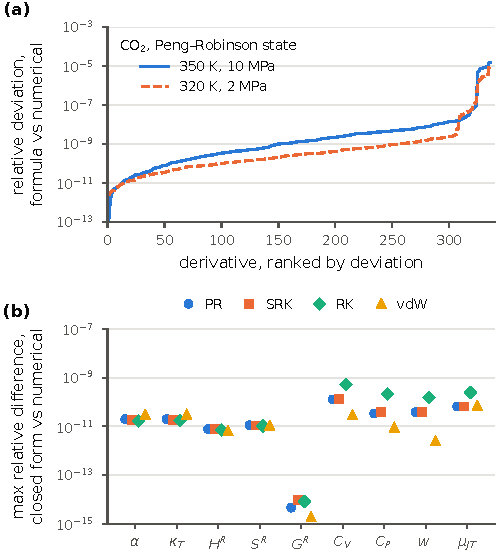
\includegraphics[width=\columnwidth]{fig2_verification}
\caption{Verification. (a) Relative deviation between each of the
\NDerivTotal{} reduced formulas and a constrained numerical derivative, ranked,
at two states of CO$_2$. (b) Largest relative difference between closed-form
and numerically obtained properties of four cubic equations.}
\label{fig:verif}
\end{figure}

\subsection{Validation against Reference Data}

\emph{Single-phase carbon dioxide.} Table~\ref{tab:val} and
Figures~\ref{fig:iso}--\ref{fig:isobar} compare the five models with the NIST
values. Over all \NNistCOtwo{} states the average absolute deviation (AAD) of
the density is \PRrhoAAD\% for PR, \RKrhoAAD\% for RK, \SRKrhoAAD\% for SRK,
\vdWrhoAAD\% for vdW, and \IGrhoAAD\% for the ideal gas. The ranking depends
on the region. Up to 4~MPa SRK is the most accurate (\SRKrhoAADlow\% against
\PRrhoAADlow\% for PR), but at 15--20~MPa its density AAD rises to
\SRKrhoAADhigh\%, whereas PR remains at \PRrhoAADhigh\%; this is the known
tendency of SRK to underpredict the density of dense fluids, which
PR was designed to reduce.\cite{Peng1976} The largest deviations of all cubic
models, \PRrhoMax\% for PR and \SRKrhoMax\% for SRK, occur at 310~K and 10~MPa,
6~K above the critical temperature (Figure~\ref{fig:map}).

Caloric and derivative properties are less accurate than density. For PR the
AAD is \PRCpAAD\% for $C_P$ (maximum \PRCpMax\% on the pseudocritical ridge),
\PRCvAAD\% for $C_V$, \PRwAAD\% for the speed of sound, and \PRmuAAD\% for the
Joule--Thomson coefficient; for SRK the corresponding values are \SRKCpAAD\%,
\SRKCvAAD\%, \SRKwAAD\%, and \SRKmuAAD\%. Along the 10~MPa isobar
(Figure~\ref{fig:isobar}) PR and SRK locate the maximum of $C_P$ correctly but
underestimate its height, and both overestimate the speed of sound near its
minimum. The vdW equation has a temperature-independent $a$, so its
$C_V^R$ is zero and its $C_V$ equals the ideal-gas value: both show the same
AAD of \vdWCvAAD\%. Enthalpy changes from the reference state (400~K,
0.1~MPa) are reproduced with an AAD of \PRdHAAD~J~mol$^{-1}$ by PR and
\SRKdHAAD~J~mol$^{-1}$ by SRK, against \IGdHAAD~J~mol$^{-1}$ when residual
contributions are neglected; entropy changes agree within
\PRdSAAD{} and \SRKdSAAD~J~mol$^{-1}$~K$^{-1}$ on average.

\emph{Nitrogen.} On the 300~K isotherm, far above the critical temperature,
density AADs are \NtwoSRKrhoAAD\% for SRK and \NtwoPRrhoAAD\% for PR, with
$C_P$ within \NtwoSRKCpAAD\% and \NtwoPRCpAAD\% and the speed of sound within
\NtwoSRKwAAD\% and \NtwoPRwAAD\% (Table~\ref{tab:val}).

\emph{Saturation.} Between 220 and 300~K the saturation pressure of CO$_2$ is
reproduced with an AAD of \PRPsatAAD\% by PR and \SRKPsatAAD\% by SRK, whose
$\alpha_c$ functions were fitted to vapor pressures, but only to \RKPsatAAD\%
by RK and \vdWPsatAAD\% by vdW (Figure~\ref{fig:sat}, Table~\ref{tab:sat}).
Saturated-liquid densities are the weak point of all cubic equations
(\PRrhoLAAD\% for PR, \SRKrhoLAAD\% for SRK). The PR enthalpy of vaporization,
a pure residual-property difference that needs no $\Cpo$, has an AAD of
\PRdHvapAAD\% with a maximum of \PRdHvapMax\% at 300~K, close to the critical
point.

\begin{table*}
\caption{Average Absolute Deviation from NIST Reference Values$^a$}
\label{tab:val}
\small
\begin{tabular}{llrrrrrrr}
\toprule
 & & \multicolumn{5}{c}{AAD (\%)} & \multicolumn{2}{c}{AAD (absolute)} \\
\cmidrule(lr){3-7}\cmidrule(lr){8-9}
$P$ (MPa) & model & $\rho$ & $C_V$ & $C_P$ & $w$ & $\mu_{JT}$ &
$\Delta h$ (J mol$^{-1}$) & $\Delta s$ (J mol$^{-1}$ K$^{-1}$) \\
\midrule
\multicolumn{9}{l}{\emph{Carbon dioxide, 310--400 K}} \\
\TabValBody
\midrule
\multicolumn{9}{l}{\emph{Nitrogen, 300 K, 1--31 MPa}} \\
\TabValNtwoBody
\bottomrule
\end{tabular}

\raggedright\footnotesize $^a$ $\Delta h$ and $\Delta s$ are changes from
400~K, 0.1~MPa (CO$_2$) or 300~K, 1~MPa (N$_2$). IG, ideal gas.
\end{table*}

\begin{figure*}
\centering
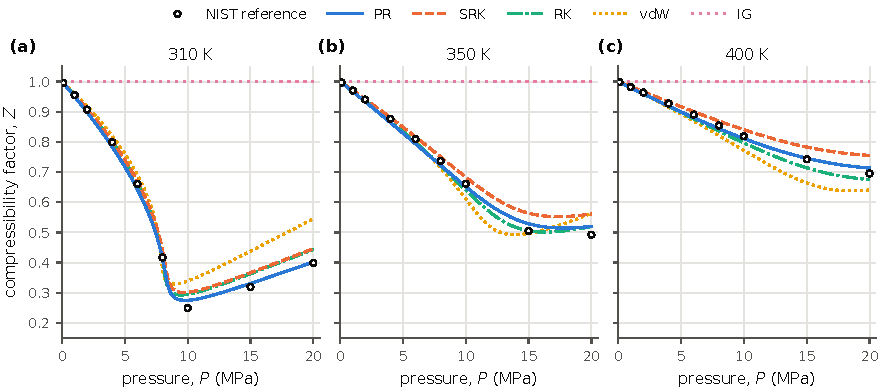
\includegraphics[width=\textwidth]{fig3_co2_isotherms}
\caption{Compressibility factor of CO$_2$ on three isotherms: five models
(lines) and NIST reference values (circles).}
\label{fig:iso}
\end{figure*}

\begin{figure*}
\centering
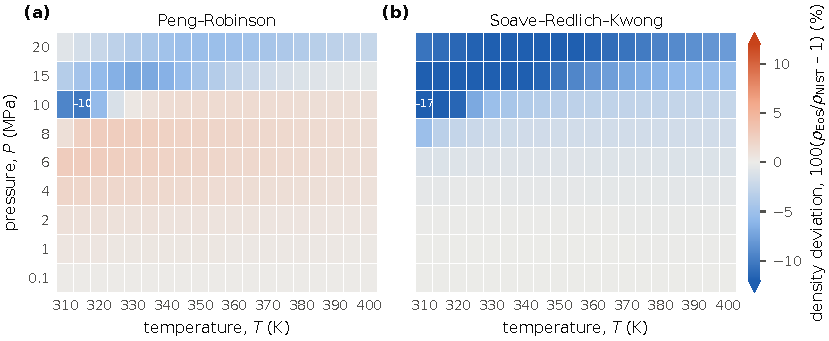
\includegraphics[width=\textwidth]{fig4_co2_density_deviation}
\caption{Percent deviation of the density of CO$_2$ from the NIST reference at
each of the \NNistCOtwo{} states for (a) Peng--Robinson and (b)
Soave--Redlich--Kwong. The number marks the largest deviation of each panel.}
\label{fig:map}
\end{figure*}

\begin{figure*}
\centering
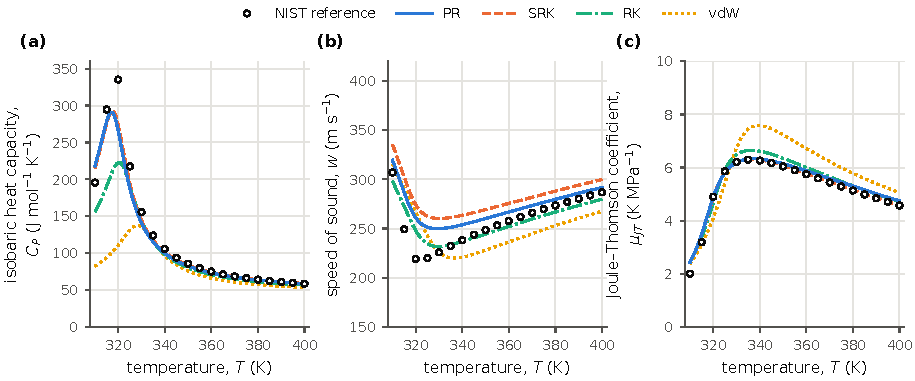
\includegraphics[width=\textwidth]{fig5_co2_isobar_10MPa}
\caption{Carbon dioxide along the 10~MPa isobar: (a) isobaric heat capacity,
(b) speed of sound, and (c) Joule--Thomson coefficient from four cubic
equations (lines) and NIST reference values (circles).}
\label{fig:isobar}
\end{figure*}

\begin{table}
\caption{Saturation of CO$_2$, 220--300 K: AAD (\%) from NIST Values}
\label{tab:sat}
\small
\begin{tabular}{lrrrr}
\toprule
model & $P^{\mathrm{sat}}$ & $\rho^{L}$ & $\rho^{V}$ & $\Delta h^{\mathrm{vap}}$ \\
\midrule
\TabSatBody
\bottomrule
\end{tabular}
\end{table}

\begin{figure}
\centering
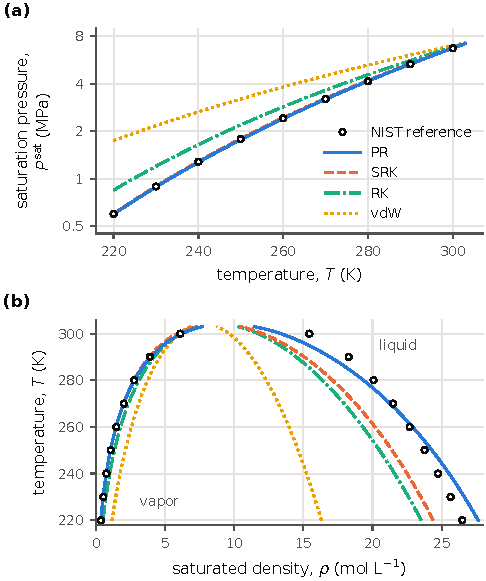
\includegraphics[width=\columnwidth]{fig6_co2_saturation}
\caption{Saturation of CO$_2$: (a) vapor pressure and (b) coexisting densities
from four cubic equations (lines) and NIST reference values (circles).}
\label{fig:sat}
\end{figure}

\emph{Tabulated input.} When the engine is given only the NIST molar volumes on
the $19\times 9$ grid, together with the $\Cpo$ correlation, enthalpy changes
between grid states are reproduced with an AAD of \TabdHAAD~J~mol$^{-1}$
(\TabdHAADlow~J~mol$^{-1}$ up to 4~MPa) and entropy changes within
\TabdSAAD~J~mol$^{-1}$~K$^{-1}$ (Table~\ref{tab:route},
Figure~\ref{fig:route}a). This is better than any cubic equation, as expected
when accurate volumes are available. In a held-out test, a table built from
every second temperature reproduces the omitted densities with an AAD of
\TabHeldrhoAAD\% (maximum \TabHeldrhoMax\%) and enthalpy changes within
\TabHelddHAAD~J~mol$^{-1}$. The route has two clear limits. First, at
\TabNRefused{} of \TabNNodes{} nodes, all at the two highest pressures and in the lower half of the temperature
range, where nine pressures cannot resolve the steep variation of $Z$, the spline
violates $\kappa_T > 0$ and the engine refuses the state; the largest enthalpy
deviation, \TabdHMax~J~mol$^{-1}$, is found in the same region. Second,
properties that need second derivatives of the table are unreliable: the AAD is
\TabCpAAD\% for $C_P$ and \TabCvAAD\% for $C_V$ (Figure~\ref{fig:route}b). Even
below 4~MPa the $C_P$ AAD is \TabCpAADlow\% with the 5~K table but
\TabHeldCpAADlow\% with the 10~K table, which is consistent with amplification
of the rounding of the five-digit tabulated volumes by an interpolating
spline. The engine issues a warning when the spline gives $C_V \le 0$, but it
does not otherwise grade the quality of second-derivative results from tables.

\begin{table}
\caption{Tabulated-Input Route for CO$_2$: AAD from NIST Values$^a$}
\label{tab:route}
\small
\setlength{\tabcolsep}{5pt}
\begin{tabular}{@{}lrrrrrr@{}}
\toprule
$P$ & $\rho$ & $C_V$ & $C_P$ & $w$ & $\Delta h$ & $\Delta s$ \\
\midrule
\TabRouteBody
\bottomrule
\end{tabular}

\raggedright $^a$ $P$ in MPa; $\rho$, $C_V$, $C_P$, $w$ in percent; $\Delta h$
in J~mol$^{-1}$; $\Delta s$ in J~mol$^{-1}$~K$^{-1}$. Refused states are
excluded.
\end{table}

\begin{figure}
\centering
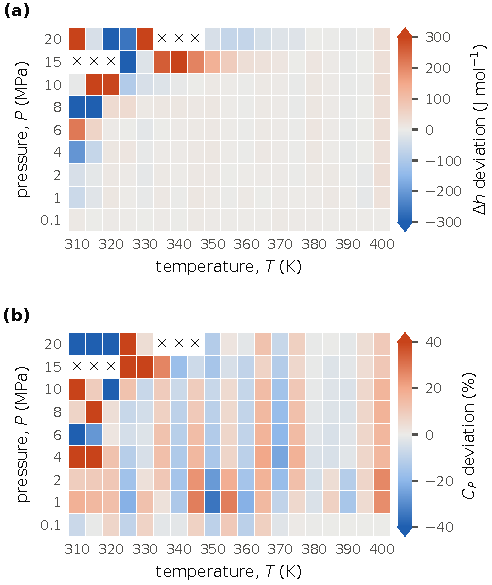
\includegraphics[width=\columnwidth]{fig7_table_route}
\caption{Tabulated-input route (all 19 temperatures) for CO$_2$: deviation from
NIST of (a) the enthalpy change from 400~K, 0.1~MPa and (b) $C_P$ at each grid
node. Crosses mark states the engine refused.}
\label{fig:route}
\end{figure}

\subsection{Worked Scenarios and Edge Cases}

Table~\ref{tab:scen} summarizes the \NScen{} scenarios distributed with the
code: \NScenOK{} complete normally, \NScenPartial{} return partial results with
the reason, \NScenIncons{} is flagged as inconsistent, and \NScenError{} are
refused with a typed error.

\emph{Inference without an EoS} (scenario 05). From stated NIST values of $V$,
$C_P$, $w$, and $\mu_{JT}$ for CO$_2$ at 350~K and 10~MPa, the rules give
$\alpha$ from $\mu_{JT}$, $\kappa_S$ from $w$, $\kappa_T$ from $\kappa_S$, and
finally $C_V = \InfCv \pm \InfCvU$~J~mol$^{-1}$~K$^{-1}$, against the NIST value
of \InfCvNist~J~mol$^{-1}$~K$^{-1}$, which was not supplied.

\emph{Tabulated process} (scenario 08). For CO$_2$ taken from 400~K, 0.1~MPa to
350~K, 10~MPa using only tabulated volumes, the engine returns
$\Delta h = \TabScendH$~J~mol$^{-1}$ and
$\Delta s = \TabScendS$~J~mol$^{-1}$~K$^{-1}$; the NIST differences are
\TabScendHNist~J~mol$^{-1}$ and \TabScendSNist~J~mol$^{-1}$~K$^{-1}$.

\emph{Saturation} (scenario 03). PR gives
$P^{\mathrm{sat}} = \SatP \pm \SatPU$~MPa at 280~K for the stated uncertainties
in $T$ and $\omega$; the NIST value is \SatPNist~MPa.

\emph{Missing data} (scenarios 06, 12, 16). With $T$, $P$, $V$, $C_P$, and
$\kappa_T$ stated, $Z$ is inferred but $C_V$ is not computable; the engine
reports that any one of $\alpha$, $\gamma$, $(\partial P/\partial T)_V$,
$\kappa_S$, $\mu_{JT}$, or the pair $(M, w)$ would suffice. A user fluid without
a $\Cpo$ model yields volumetric and residual properties and a statement that
caloric properties need $\Cpo(T)$.

\emph{Inconsistent input} (scenario 07). A stated $C_V$ larger than $C_P$ is
rejected twice: it disagrees with $C_P - TV\alpha^2/\kappa_T$ by more than the
tolerance, and it violates $C_P \ge C_V$.

\emph{Out of range} (scenarios 09 and 13). A request at 450~K against a table
ending at 400~K, and a state at 250~K when the $\Cpo$ correlation starts at
298~K, are refused with the valid range stated.

\emph{Units} (scenarios 10, 11, and 14). A pressure given in kelvin and a
temperature without a unit are refused; mixed input in degrees Celsius and bar
is converted, and output is returned in requested units.

\emph{Undefined derivative} (scenario 17). For an ideal gas the engine returns
$(\partial T/\partial P)_H = 0$ and reports that $(\partial P/\partial T)_H$ is
singular.

\begin{table*}
\caption{Scenarios Distributed with the Engine and Their Outcomes}
\label{tab:scen}
\small
\begin{tabular}{llll}
\toprule
no. & type & content & outcome \\
\midrule
\TabScenBody
\bottomrule
\end{tabular}
\end{table*}

\subsection{Uncertainty Results}

For the PR state of CO$_2$ at 350~K and 10~MPa with $u(T) = 0.1$~K,
$u(P) = 0.01$~MPa, $u(T_c) = 0.015$~K, $u(P_c) = 0.003$~MPa, and
$u(\omega) = 0.001$ (illustrative values chosen by us, not taken from the
literature), the engine gives $C_P = \OneCp \pm \OneCpU$~J~mol$^{-1}$~K$^{-1}$
and $\mu_{JT} = \OneMu \pm \OneMuU$~K~MPa$^{-1}$. For the process from 400~K,
0.1~MPa to 320~K, 15~MPa (Table~\ref{tab:budget}, Figure~\ref{fig:unc}a),
$\Delta h = \TwodH \pm \TwodHU$~J~mol$^{-1}$, with \TwodHShareTtwo\% of the
variance due to the final temperature and \TwodHShareOmega\% to the acentric
factor, and $\Delta s = \TwodS \pm \TwodSU$~J~mol$^{-1}$~K$^{-1}$, with
\TwodSSharePone\% due to the initial pressure through the term $-R\ln P$ and
\TwodSShareTtwo\% to the final temperature. The dominant input therefore
depends on the output: near the pseudocritical region the final temperature
controls the enthalpy, whereas the low initial pressure, known only to 1\%,
controls the entropy. In the inference scenario the uncertainty of the
inferred $C_V$ comes mainly from the stated $C_P$ (\InfCvShareCp\%) and
$\mu_{JT}$ (\InfCvShareMu\%) (Figure~\ref{fig:unc}b). Monte Carlo and
first-order standard uncertainties agree within a ratio of \MCRatioMin{} to
\MCRatioMax{} for the \MCN{} outputs of the two EoS scenarios, so that
linearization is adequate for these input uncertainties.

These uncertainties must not be read as accuracies. At 350~K and 10~MPa the
propagated $u(C_P)$ is \OneCpU~J~mol$^{-1}$~K$^{-1}$, whereas the PR value
differs from the NIST value of \OneCpNist~J~mol$^{-1}$~K$^{-1}$ by more than
ten times that amount; the PR density is \OneRho~mol~L$^{-1}$ against
\OneRhoNist~mol~L$^{-1}$. Model error dominates wherever a cubic equation is
used at elevated density.

\begin{table*}
\caption{Uncertainty Budget for the Process of Scenario 02 (CO$_2$, PR)$^a$}
\label{tab:budget}
\small
\begin{tabular}{lrrrrrrrrr}
\toprule
 & & & \multicolumn{7}{c}{share of variance (\%)} \\
\cmidrule(lr){4-10}
output & value & $u$ & $T_1$ & $P_1$ & $T_2$ & $P_2$ & $T_c$ & $P_c$ & $\omega$ \\
\midrule
\TabBudgetBody
\bottomrule
\end{tabular}

\raggedright\footnotesize $^a$ $u(T_1) = u(T_2) = 0.1$~K, $u(P_1) = 0.001$~MPa,
$u(P_2) = 0.015$~MPa, $u(T_c) = 0.015$~K, $u(P_c) = 0.003$~MPa,
$u(\omega) = 0.001$.
\end{table*}

\begin{figure*}
\centering
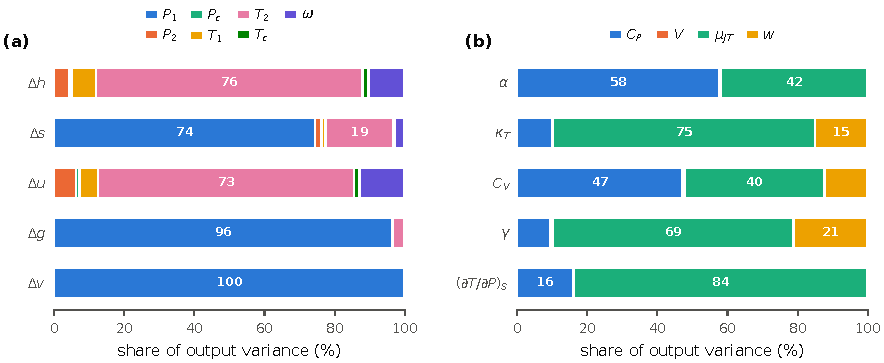
\includegraphics[width=\textwidth]{fig8_uncertainty_budget}
\caption{Share of the output variance contributed by each uncertain input:
(a) property changes of the PR process of scenario 02 and (b) quantities
inferred from stated measurements in scenario 05.}
\label{fig:unc}
\end{figure*}

\subsection{Limitations and Failure Modes}

The engine treats a pure, closed, simple compressible fluid in a single phase
per state. Mixtures, chemical reaction, two-phase states at a specified
quality, and solid phases are outside its scope, and only first derivatives are
reduced. The fluid database contains two substances; others require the user to
supply constants. The cubic equations are inaccurate where they are known to
be: close to the critical point,
for liquid densities, and for second-derivative properties
(Table~\ref{tab:val}); the vdW and RK equations should not be used for
saturation. The $\Cpo$ correlation for CO$_2$ starts at 298~K, so caloric
properties of colder CO$_2$ are refused unless the user allows extrapolation or
supplies another correlation; single-phase liquid states were therefore not
validated. The tabulated route interpolates without smoothing, cannot assess
whether a grid is fine enough, and gives unreliable second-derivative
properties from rounded data. Uncertainty propagation assumes uncorrelated
inputs and excludes model error. The normal form of the symbolic reducer is not
guaranteed to be the shortest expression. The reference data were transcribed
by hand, with the integrity test described above. The tabulated-$\Cpo$ input
path was exercised by one scenario only, and no comparison with experimental
measurements, as opposed to reference equations, was made.

\section{Conclusion}

A compact engine for the calculus of thermodynamics has been presented. It
reduces all \NDerivTotal{} first derivatives of eight state variables exactly,
decides computability from the symbols a result needs, explains what is missing
or contradictory, accepts stated, tabulated, inferred, and parameterized inputs
on the same footing, and attaches an uncertainty budget to its results. The
mathematics was verified against independent numerical differentiation to
$\DerivMaxDevSC$ or better and the closed-form EoS results against a
model-independent scheme to $\ClosedNumMax$. Validation against NIST data shows
what cubic equations deliver for CO$_2$ at 310--400~K and up to 20~MPa: densities
within \PRrhoAAD\% on average for PR, vapor pressures within \PRPsatAAD\%, and
caloric properties that degrade toward the critical region. With tabulated
volumes the engine reproduces enthalpy changes within \TabdHAAD~J~mol$^{-1}$ on
average but cannot be trusted for heat capacities. The engine complements, and
does not replace, reference-quality property libraries; its value lies in
making the chain from data to derivative explicit and checkable.

\section*{Data and Software Availability}

The code package, all scenario input files, all output files, the NIST
reference values used, and the script that regenerates every figure, table, and
number of this paper accompany the manuscript in the folders \texttt{Codes}
and \texttt{Data}. An interactive web version of the engine is included in
\texttt{Codes/website}, and a command-line dialogue that prompts for missing
data is run with \texttt{python -m thermocalculus ask}.

\begin{acknowledgement}
[TO FILL BY THE AUTHORS: course, instructor, and any funding.]
[AI-USE DISCLOSURE, TO CONFIRM AND EDIT BY THE AUTHORS, as required by the
journal: An AI assistant (Claude, Anthropic) was used to write the engine code,
run the calculations, prepare the figures, and draft the text of this
manuscript. The authors reviewed and take responsibility for all content.]
\end{acknowledgement}

\bibliography{references}

\begin{tocentry}
\centering
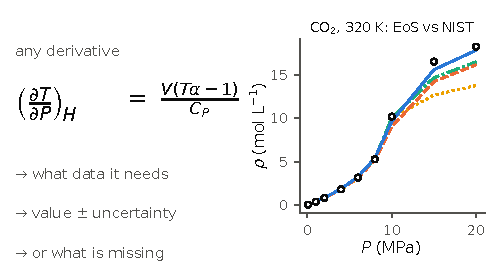
\includegraphics[width=8.0cm,height=4.3cm,keepaspectratio]{toc_graphic}
\end{tocentry}

\end{document}
